%%%%%%%%%%%%%%%%%%%%%%%%%%%%%%%%%%%%%%%%%
% Structured General Purpose Assignment
% LaTeX Template
%
% This template has been downloaded from:
% http://www.latextemplates.com
%
% Original author:
% Ted Pavlic (http://www.tedpavlic.com)
%
% Note:
% The \lipsum[#] commands throughout this template generate dummy text
% to fill the template out. These commands should all be removed when
% writing assignment content.
%
%%%%%%%%%%%%%%%%%%%%%%%%%%%%%%%%%%%%%%%%%

%----------------------------------------------------------------------------------------
%	PACKAGES AND OTHER DOCUMENT CONFIGURATIONS
%----------------------------------------------------------------------------------------

\documentclass{article}

\usepackage{multirow}
\usepackage{amssymb}
\usepackage[fleqn]{amsmath}
\usepackage{url}

\usepackage{fancyhdr} % Required for custom headers
\usepackage{lastpage} % Required to determine the last page for the footer
\usepackage{extramarks} % Required for headers and footers
\usepackage{graphicx} % Required to insert images
\usepackage{lipsum} % Used for inserting dummy 'Lorem ipsum' text into the template

% Margins
\topmargin=-0.45in
\evensidemargin=0in
\oddsidemargin=0in
\textwidth=6.5in
\textheight=9.0in
\headsep=0.25in

\linespread{1.1} % Line spacing

% Set up the header and footer
\pagestyle{fancy}
\lhead{\hmwkAuthorName} % Top left header
\chead{\hmwkClass\ : \hmwkTitle} % Top center header
\rhead{\firstxmark} % Top right header
\lfoot{\lastxmark} % Bottom left footer
\cfoot{} % Bottom center footer
\rfoot{Page\ \thepage\ of\ \pageref{LastPage}} % Bottom right footer
\renewcommand\headrulewidth{0.4pt} % Size of the header rule
\renewcommand\footrulewidth{0.4pt} % Size of the footer rule

\setlength\parindent{0pt} % Removes all indentation from paragraphs

%----------------------------------------------------------------------------------------
%	DOCUMENT STRUCTURE COMMANDS
%	Skip this unless you know what you're doing
%----------------------------------------------------------------------------------------

% Header and footer for when a page split occurs within a problem environment
\newcommand{\enterProblemHeader}[1]{
\nobreak\extramarks{#1}{#1 continued on next page\ldots}\nobreak
\nobreak\extramarks{#1 (continued)}{#1 continued on next page\ldots}\nobreak
}

% Header and footer for when a page split occurs between problem environments
\newcommand{\exitProblemHeader}[1]{
\nobreak\extramarks{#1 (continued)}{#1 continued on next page\ldots}\nobreak
\nobreak\extramarks{#1}{}\nobreak
}

\setcounter{secnumdepth}{0} % Removes default section numbers
\newcounter{homeworkProblemCounter} % Creates a counter to keep track of the number of problems

\newcommand{\homeworkProblemName}{}
\newenvironment{homeworkProblem}[1][Problem \arabic{homeworkProblemCounter}]{ % Makes a new environment called homeworkProblem which takes 1 argument (custom name) but the default is "Problem #"
\stepcounter{homeworkProblemCounter} % Increase counter for number of problems
\renewcommand{\homeworkProblemName}{#1} % Assign \homeworkProblemName the name of the problem
\section{\homeworkProblemName} % Make a section in the document with the custom problem count
\enterProblemHeader{\homeworkProblemName} % Header and footer within the environment
}{
\exitProblemHeader{\homeworkProblemName} % Header and footer after the environment
}

\newcommand{\problemAnswer}[1]{ % Defines the problem answer command with the content as the only argument
\noindent\framebox[\columnwidth][c]{\begin{minipage}{0.98\columnwidth}#1\end{minipage}} % Makes the box around the problem answer and puts the content inside
}

\newcommand{\homeworkSectionName}{}
\newenvironment{homeworkSection}[1]{ % New environment for sections within homework problems, takes 1 argument - the name of the section
\renewcommand{\homeworkSectionName}{#1} % Assign \homeworkSectionName to the name of the section from the environment argument
\subsection{\homeworkSectionName} % Make a subsection with the custom name of the subsection
\enterProblemHeader{\homeworkProblemName\ [\homeworkSectionName]} % Header and footer within the environment
}{
\enterProblemHeader{\homeworkProblemName} % Header and footer after the environment
}

%----------------------------------------------------------------------------------------
%	NAME AND CLASS SECTION
%----------------------------------------------------------------------------------------


%----------------------------------------------------------------------------------------
%	TITLE PAGE
%----------------------------------------------------------------------------------------

\title{
\vspace{2in}
\textmd{\textbf{\hmwkClass:\ \hmwkTitle}}\\
\normalsize\vspace{0.1in}\small{Due\ on\ \hmwkDueDate}\\
\vspace{3in}
}

\author{\textbf{\hmwkAuthorName}}
\date{} % Insert date here if you want it to appear below your name



\usepackage{clrscode}
\usepackage{enumerate}
\newcommand{\hmwkTitle}{Assignment\ \#6} % Assignment title
\newcommand{\hmwkDueDate}{April\ 13,\ 2016} % Due date
\newcommand{\hmwkClass}{Algorithms} % Course/class
\newcommand{\hmwkAuthorName}{Zhaoyang Li (2014013432)} % Your name
%----------------------------------------------------------------------------------------

\begin{document}

\maketitle

%----------------------------------------------------------------------------------------
%	TABLE OF CONTENTS
%----------------------------------------------------------------------------------------

\setcounter{tocdepth}{1} % Uncomment this line if you don't want subsections listed in the ToC

\newpage
\tableofcontents
\newpage

%----------------------------------------------------------------------------------------
%	PROBLEM 1
%----------------------------------------------------------------------------------------


\begin{homeworkProblem}

CLRS Exercises 32.4-8.

\problemAnswer{


\begin{codebox}
\Procname{\proc{Compute-Transition-Function-Fast($P$, $\Sigma$)}}

\li $\pi \gets$ \proc{Compute-Prefix-Function($P$)}
\li $m \gets P.length$
\li \For each character $a\in\Sigma$
\li      \Do $\delta(0, a) = 0$ \End
\li \For $q = 0$ \To $m$
\li            \Do \For each character $a\in\Sigma$
\li                 \Do $\delta(q, a) = \delta(\pi[q], a)$
\li                     \If $q\neq m$ and $P[q+1]=a$
\li                            \Then $\delta(q, a) = q+1$  \End
                        \End
                    \End
                \End
\li \Return $\delta$
\end{codebox}


\paragraph{Timing} Lines 1 to 2 takes $\Theta(m)$ time. Lines 3 to 4 takes $\Theta(|\Sigma|)$ time. The double-loop starting from lines 5 takes $\Theta(m|\Sigma|)$ time. Therefore, total running time $T\in O(m|\Sigma|)$.

\paragraph{Correctness} We'll prove that if $q=m$ or $P[q+1]\neq a$, then $\delta(q,a)=\delta(\pi[q],a)$.

Let's look at the definition of the prefix function $\pi$,

$$\pi[q]=\max\{k: k<q\ \text{and}\ P_k\sqsupset P_q\}$$

Meanwhile, our transition function is supposed to meet the following equation
$$\delta(q, a) = \sigma(P_q a),\ \text{where}\ \sigma(x)=\max\{k:P_k\sqsupset x\}$$

Now everything is ready, and all we need is an east wind.

\begin{equation}
\begin{aligned}
\delta(\pi[q],a) &= \delta(\max\{k: k<q\ \text{and}\ P_k\sqsupset P_q\},a) \\
&=\delta(\sigma(P_q), a) \\
&=\sigma(P_{\sigma(P_q)}a)\\
&=\sigma(P_q a)\\
&=\delta(q, a)
\end{aligned}
\end{equation}

QED.
}
\end{homeworkProblem}


%----------------------------------------------------------------------------------------
%	PROBLEM 2
%----------------------------------------------------------------------------------------


\begin{homeworkProblem}

CLRS Problems 32-1. String matching based on repetition factors.


\problemAnswer{
a. The repetition factor is related to the prefix function introduced in KMP. As a matter of fact, we may prove the following lemma:

$$\forall i, \pi[i]=i-\frac{i}{\rho(P_i)}$$
\begin{codebox}
\Procname{\proc{Compute-Repetition-Factor($P$)}}

\li let $\rho[1...m]$ be a new array, in which 
\li $\rho[1]\gets1$
\li $\pi \gets$ \proc{Compute-Prefix-Function($P$)}
\li \For $i = 2$ \To $P.length$
\li            \Do \If $i -\pi[i] = \frac{\pi[i]}{\rho[\pi[i]]}$
\li                            \Then $\rho[k]\gets\rho[\pi[i]]+1$  
\li                             \Else $\rho[k]\gets1$ \End
            \End
\li \Return $\rho$
\end{codebox}
Running time $\Theta(m)+\Theta(m)=\Theta(m)$, where $m$ is the length of the pattern string $P$.
}\problemAnswer{
b.
}\problemAnswer{
c. 

\paragraph{Timing} Consider line 12 where $s$ is increased. Suppose this line is executed $t$ times, each time $q=q_i$. Since $s$ is increased from $0$ to $n-m$, we know that

$$\sum_{i=1}^{t}\frac{q_i}{k} = n-m$$

Now look at line 8. Since $q$ is increased by $1$ at a time and decreased only on line 13, we know that lines 7-10 are executed no more than $\sum_{i=1}^t q_i$ times.

Each time we enters the loop body, either $q$ is decreased or $s$ is increased (otherwise, the loop becomes endless). Thus, times of the loop body being entered
\begin{equation}
\begin{aligned}
\sum_{i=1}^t q_i + t 
&= k\times(n-m)+t \\
&= \left(1+\rho^*(P)\right)\times(n-m)+t \\
&=O\left(\rho^*(P)n+m\right)
\end{aligned}
\end{equation}

Running time $T\in O\left(\rho^*(P)n+m\right)$.
}
\end{homeworkProblem}

%----------------------------------------------------------------------------------------
%	PROBLEM 3
%----------------------------------------------------------------------------------------


\begin{homeworkProblem}

Compare string matching algorithms Brute-Force, KMP and BM.

\problemAnswer{
\subsection{Implementation and environment}
\paragraph{Language} The C++ programming language
\paragraph{IDE} Visual Studio 2015 and Qt Creator 3.6.1
\paragraph{Compiling} Desktop Qt 5.6.0, MSVC2015 64bit Release
\paragraph{OS} Windows 10 Education, Build 10586
\paragraph{Hardware} Intel Core i7-6600U @ 2.60GHz, 16GB LPDDR3, ThinkPad X1 Carbon 20FB
}\problemAnswer{
\subsection{Verification of correctness}
\paragraph{}Code written in reference\footnote{http://www-igm.univ-mlv.fr/~lecroq/string/} to a trust-worthy academic institute.

\paragraph{}Correctness of the code is verified by comparing the respective results from the three algorithms for consistency. All test samples are passed.
}\problemAnswer{
\subsection{Timing}
There are several factors that may influence running-time of string matching algorithms, including
\begin{itemize}
\item text style (size of set of possible characters, repetition factor, etc)
\item length of pattern string
\item length of text string
\item ...
\end{itemize}

So we need to do several sets of experiments here.

In order to be more precise, all timing are done by repeating the algorithm several times and calculating an average running-time.
\subsubsection{Text style?}
\paragraph{} Many of my classmates use randomly generated text as their string to be searched in, as far as I know. I doubt if it's a reasonable thing to do. So I managed to collect three blocks of text which are in different styles -

\begin{itemize}
\item C source code of the XV6 operating system
\item full text of an English novel The Wonderful Wizard of Oz
\item randomly generated text, full of CAPITALIZED English letters
\end{itemize}
each of which are made to have an approximate length of $10^6$, by performing Ctrl+C and Ctrl+V if necessary.

\paragraph{}Results illustrated as below.
}\problemAnswer{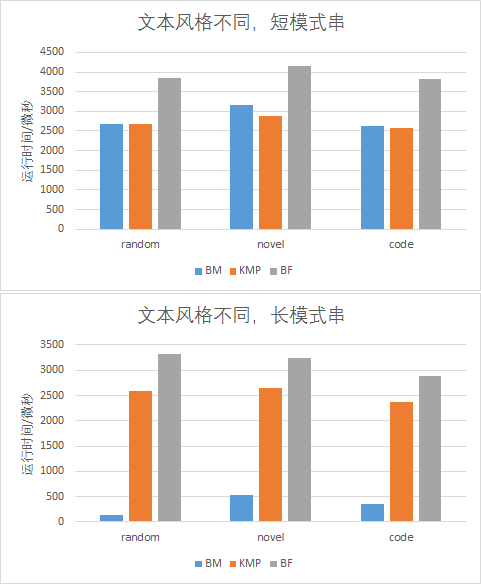
\includegraphics{text-style}
}\problemAnswer{
\paragraph{}It can be concluded that style of the text (randomly generated or not) has no affect on timing comparison. In another word, the algorithm that takes the longest time always takes the longest time. Thus, it's reasonable to use randomly generated text to represent general cases. That's exactly what I did hereinafter.

\paragraph{} Also, BM has more advantage with longer patterns. I did more experiments to confirm this.
}\problemAnswer{
\subsubsection{Pattern length}
\paragraph{} For BF and KMP, pattern length has little affect on running-time of the algorithm. However, as length of pattern grows, running-time of BM reduces significantly.
}\problemAnswer{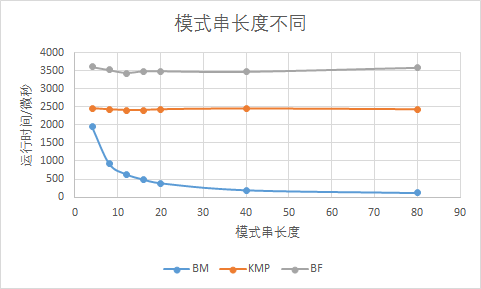
\includegraphics{pattern-length}
}\problemAnswer{
\subsubsection{Text length}
\paragraph{}Finally, let's take a look at how running-time grows as length of the text string grows.

\paragraph{}Perfect linearity, as expected. BF $>$ KMP $>$ BM, as expected.
}\problemAnswer{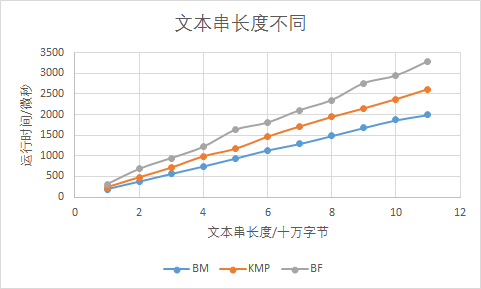
\includegraphics{text-length}
}
\end{homeworkProblem}



%----------------------------------------------------------------------------------------

\end{document}
